\usetikzlibrary{shadows,arrows}
% Define the layers to draw the diagram
\pgfdeclarelayer{background}
\pgfdeclarelayer{foreground}
\pgfsetlayers{background,main,foreground}
 
% Define block styles  
\tikzstyle{rectangle}=[draw, fill=blue!20, text width=6.0em, text centered,
  minimum height=1.5em,drop shadow]
\tikzstyle{practica} = [rectangle, text width=8em, minimum width=10em,
  minimum height=3em, rounded corners, drop shadow]

\tikzstyle{circle}=[draw, fill=green!20, text width=6.0em, text centered,
  minimum height=1.5em,drop shadow]
\tikzstyle{interface} = [circle, text width=8em, minimum width=10em,
  minimum height=3em, rounded corners, drop shadow]
 
\tikzstyle{texto} = [above, text width=6em, text centered]
\tikzstyle{linepart} = [draw, thick, color=black!50, -latex', dashed]
\tikzstyle{line} = [draw, thick, color=black!50, -latex']
 
% Define distances for bordering

\newcommand{\practica}[2]{node (p#1) [practica] {#2}}
\newcommand{\implemented}[2]{node (p#1) [interface] {#2}}

% Draw background
\newcommand{\background}[5]{%
  \begin{pgfonlayer}{background}
    % Left-top corner of the background rectangle
    \path (#1.west |- #2.north)+(-0.5,0.5) node (a1) {};
    % Right-bottom corner of the background rectanle
    \path (#3.east |- #4.south)+(+0.5,-0.25) node (a2) {};
    % Draw the background
    \path[fill=yellow!20,rounded corners, draw=black!50, dashed]
      (a1) rectangle (a2);
    \path (a1.east |- a1.south)+(0.8,-0.3) node (u1)[texto]
      {\scriptsize\textit{#5}};
  \end{pgfonlayer}}

\newcommand{\transreceptor}[3]{%
  \path [linepart] (#1.east) -- node [above]
    {\scriptsize Transreceptor #2} (#3);}

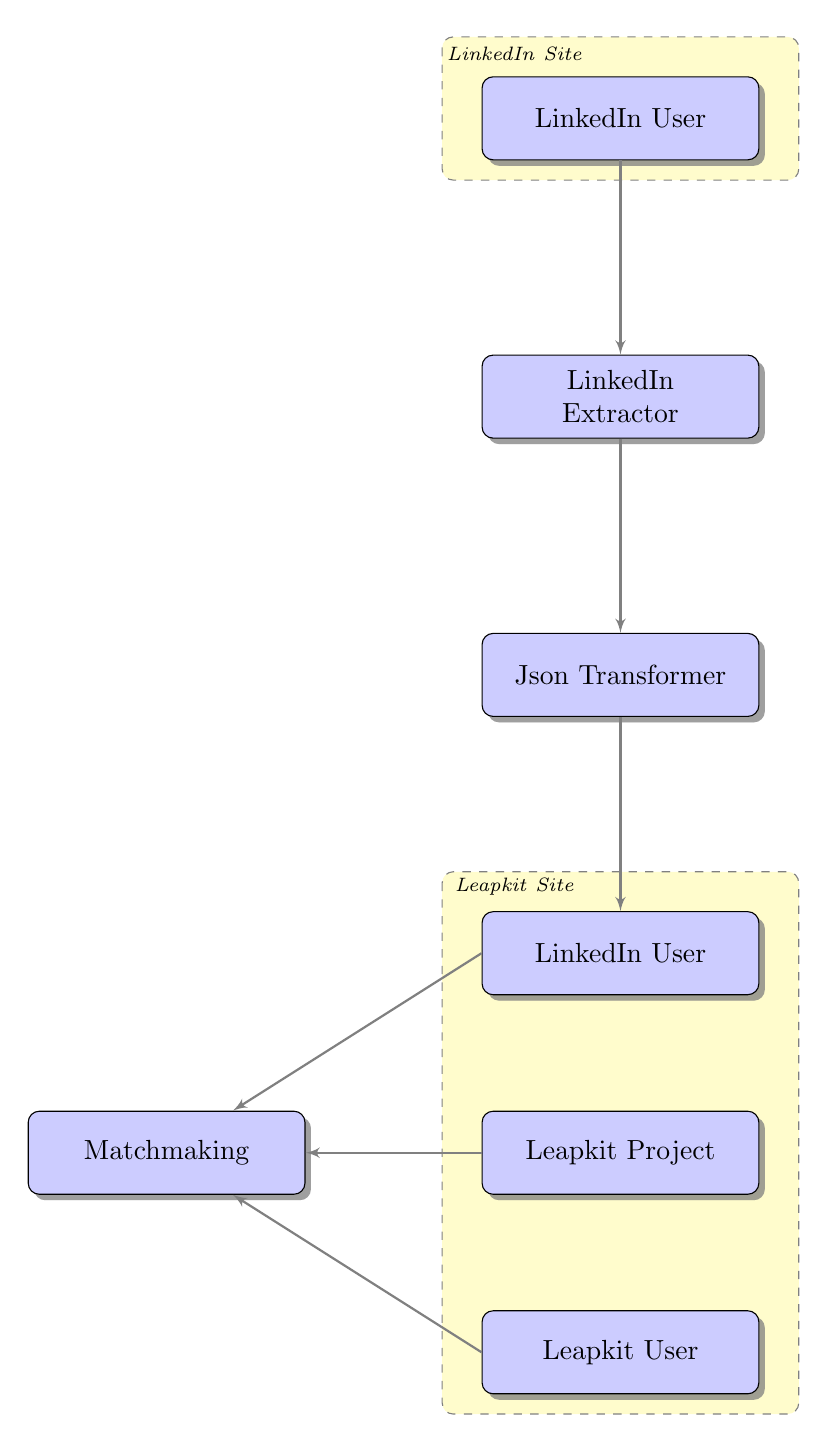
\begin{tikzpicture}


% Draw diagram elements
\path                          \practica{1}{LinkedIn User};

\path (p1.south) +( 0.0,-3.0) \practica{2}{LinkedIn Extractor};
\path (p2.south) +( 0.0,-3.0) \practica{3}{Json Transformer};


\path (p3.south)+(0.0,-3.0) \practica{6}{LinkedIn User};
\path (p6.south)+(0.0,-2.0) \practica{7}{Leapkit Project};
\path (p7.south)+(0.0,-2.0) \practica{8}{Leapkit User};
 
\path (p7.west)+(-4.0,0.0) \practica{9}{Matchmaking};

% Draw arrows between elements
\path [line] (p1.south) -- node [above] {} (p2.north);

\path [line] (p2.south) -- node [above] {} (p3.north);

\path [line] (p3.south) -- node [above] {} (p6.north);
\path [line] (p6.west) -- node [above] {} (p9);
\path [line] (p7.west) -- node [above] {} (p9);
\path [line] (p8.west) -- node [above] {} (p9);

\background{p1}{p1}{p1}{p1}{LinkedIn Site}
\background{p6}{p6}{p8}{p8}{Leapkit Site}

\end{tikzpicture}
